\chapter{Technischen Grundlagen} \label{Theoretische Grundlagen}
Im diesem Kapitel werden die Technischen Grundlagen der verwendeten Technologien im einzelnen betrachtet.
\todo{Leser klar machen warum die einzelnen dinge beschrieben werden}
\todo{mehr Bilder zur erklärung, auchmit bezug auf die arbeit}
\section{HTML 5}
In dieser Sektion wird nicht auf HTML5 allgemein eingegangen, es werden ausschließlich die Elemente erläutert welche verwendet wurden und durch die momentan neuste Spezifikation der Hypertext Markup Language spezifiziert sind. Ganz allgemein ist zu sagen, dass es HTML5 erlaubt interaktivere Anwendungen zu gestalten. HTML ist dabei die Sprache die verwendet wird, um das Aussehen der Seite zu spezifizieren. In der entwickelten Anwendung wurde sie in der Webanwendung des Therapeuten und auch in der Mobilen App für den Patienten verwendet.

Das \textbf{nav} Element wurde in der Therapeuten Webanwendung verwendet um die Navigationsleiste zu spezifizieren. Hier sind nur die Links zu den einzelnen Hauptseiten definiert. Durch die in den meisten Browsern automatisch verwendete CSS Eingenschaft \textit{display : block} wird diese als Box über die gesamte breite der Seite angezeigt \cite{SELFHTMLD16}. Durch Twitter Bootstrap bekommt die Navigationsleiste ihr aussehen und weitere Funktionalität.

Bei den verschiedenen \textbf{input} Elementen in beiden Clients konnte mittels HTML5 spezifiziert werden welche Art von Eingabe in dem jeweiligen Textfeld erwartet wird. Dies wurde verwendet um die Eingabe des Geburtsdatums des Patienten mit Hilfe des Input-Typs \textbf{date} zu erleichtern. Mittels des Input-Typs \textbf{email} wird automatisch kontrolliert ob die eingegebene E-Mail Adresse dem Standard für diese entspricht.

\section{Daten beim Aufrufen oder wechseln einer Seite übergeben}
Bei Webanwendungen wie die im Rahmen dieser Arbeit entstandenen, ist es immer wieder nötig, zum Beispiel beim Wechsel zu einer anderen Seite Daten an diese zu übergeben. Dies kann auf verschiedenen Wegen geschehen.

Bei kleiner Datenmengen wie Beispielsweise einer Id wird diese meinst in der URL übergeben. Diese wird dann an die eigentlich aufzurufende URL (z.B. http://eine.ip/index.html) nach einem \textbf{?} angehängt.
Die aufzurufende URL hat dann Beispielsweise die Form \\ \textit{http://eine.ip/index.html?patientId=eine1Id}.
Wird die Seite auf diese Art aufgerufen kann die Variable patientId dann von dieser ausgelesen werden. Soll mehr wie eine Variable übergeben werden,können diese mit dem \textbf{\&} Zeichen an einander angehängt werden.

Wenn größere Datenmengen zu übertragen sind, werden diese innerhalb des HTTP Objektes in dessen Rumpf übergeben. Dies wird in dieser Anwendung Beispielsweise verwendet, wenn nach der Anfrage an den Datenbank Server dessen Antwort mit dem Objekt im JSON Format Beispielsweise eines Patienten zurück gesendet wird.

 Angular, Mongoose MongoDB
 Client Webanwendungen, single page application Bootstrap
 Zentralisierung der Daten (Sicherheit)
 
 Android debug bridge ADB
 
\section{REST-Service}
Um eine gemeinsame Datenbasis zwischen den beiden Clients für Therapeut und Patient zu schaffen bietet der im Rahmen dieser Arbeit entwickelte Server einen REST-Service zum abrufen der in der Datenbank gespeicherten Daten an. Mit dessen Hilfe können die Daten zu den Patienten, Aufgaben und Fragebögen über das Internet mittels HTTP Anfragen auf jedem Gerät abgerufen und verändert werden. Das Programmierparadigma eines REST-Services soll dabei verschiedenen Prinzipien folgen.

Zum einen soll dieser Service \textbf{Zustandslos} sein. Bei jedem Aufruf müssen somit alle zum verstehen der Nachricht nötigen Daten übermittelt werden.
Ein weiteres Prinzip ist die \textbf{Adressierbarkeit} der einzelnen Ressourcen, welches in dieser Anwendung durch die einzigartige Id jedes Objekts realisiert wurde.
\subsection{Die HTTP-Methoden}
Um mit dem Service zu interagieren stehen verschiedene HTTP-Methoden zu Verfügung. Welche hier kurz erklärt werden.
\paragraph{HTTP-GET}
Mittels HTTP-GET wird dem Server signalisiert, dass Daten abgerufen werden wollen. Hierbei kann eine allgemeine Anfrage gestellt werden um alle vorhandenen Daten zu erhalten oder mittels der unter Adressierbarkeit angesprochen Id ein bestimmtes Objekt angefordert werden.
\paragraph{HTTP-POST}
Diese Methode wird verwendet um ein neues Objekt in der Datenbank anzulegen. Der Server antwortet hierbei mit dem Angelegten Objekt welches die vom Server erzeugte, einzigartige Id enthält.
\paragraph{HTTP-PUT}
Mit Hilfe der PUT-Methode kann ein auf dem Server vorhandenes Objekt verändert werden, hierbei muss die Id bekannt sein und übermittelt werden.
\paragraph{HTTP-DELETE}
Durch diese Methode kann ein Objekt anhand seiner Id auf dem Server gelöscht werden.

\section{Sicherheit}
Da es sich bei den ausgetauschen Daten um brisante Patientendaten handelt sollte das Thema Sicherheit sehr groß geschrieben werden. Da es jedoch den Rahmen dieser Arbeit überzogen hätte, wird es nur theoretisch betrachtet und wurde während der Implementierung völlig außer Acht gelassen. Bevor die Plattform mit realen Daten verwendet wird muss in jedem Fall zuerst verhindert werden, dass unbefugte auf die Daten der Patienten zugreifen können. In diesem Abschnitt sollen Ideen und Anregungen gegeben werden wie dies bewerkstelligt werden kann. 
Da in einem REST-Service nicht von Haus aus Schutzmechanismen eingebaut sind liegt es in der Hand des Entwicklers die oben beschriebenen, unsicheren HTTP Methoden vor dem Zugriff durch unberechtigte zu schützen.
\subsection{Verschlüsselung der Daten}
Der erste Schritt um vor allem die Daten der Patienten zu sichern ist es, die Verbindung zwischen Server und Client zu verschlüsseln. 
\subsection{OAuth}


\section{BPMN-IO}
Um dem Therapeuten innerhalb des für ihn konzipierten Clients die Möglichkeit zu geben eigene Fragebögen zu erstellen wurde versucht ein Modul zu finden das sich einfach in die Anwendung integrieren lässt. Es gibt einige Module für das Angular Framework, welche eine Oberfläche bieten um Fragebögen zu erstellen. Jedoch war eine der Voraussetzungen, dass die Fragen von der Antwort der vorigen Frage abhängig sein sollte. Keines der gefundenen Framework bot jedoch dieses Feature. Somit wurde untersucht welche anderen Anwendungen es gibt, welche für diesen Zweck angepasst werden könnten.
\subsection{Aufbau der exportierten XML Datei}
 
 

\section{Anwendungsentwicklung} \todo{bezug auf die Anwedung}
Am Anfang jeder mobilen Anwendung steht die Entscheidung auf welchen Geräten diese laufen soll. Natürlich besteht die Möglichkeit eine Anwendung nativ für eine bestimmte Plattform zu entwickeln.

Um die Anwendung auf anderen Plattformen zu bringen ist es dann jedoch nötig diese praktisch neu für diese zu implementieren. Aus diesem Dilemma heraus entstanden verschiedenen Frameworks die es dem Entwickler möglich machen, direkt für mehrere Plattformen zu entwickeln. Hierdurch ist es dann möglich seinen Code nur einmal zu schreiben und diesen dann direkt, mithilfe eines Frameworks, wie zum Beispiel eines Browsers auf den verschiedene Plattformen laufen zu lassen.

Es müssen dann nur einige wenige Abschnitte des Codes nativ für die jeweilige Plattform geschrieben werden, wenn diese nicht verallgemeinerbar sind bzw. nicht schon durch eine Bibliothek vereinheitlicht wurden. Ein Beispiel wäre hier der Zugriff auf Dateien, hier ist es nicht möglich den Zugriff direkt zu verallgemeinern, da die verschiedenen Betriebssysteme unterschiedliche Dateisysteme Verwenden.

Eine der Grundvoraussetzungen dieser Arbeit sollte die Verfügbarkeit für möglichst viele Patienten sein. Aus diesem Grund wurde vorab untersucht durch welche Techniken es möglich ist, die Hürde der vielen verschiedenen Endgeräte und damit verbundenen Betriebssysteme umgehen zu können. Durch die enge Bindung der Therapeutensoftware an den Server viel die Wahl von vorn herein auf eine sogenannte \textbf{Single-Page-Application} in Form einer Website.


\subsection{Anwendungsentwicklung für mobile Geräte}
Das größte Problem der Anwendungsentwicklung für Smartphones ist, dass es viele verschiedene mobile Betriebssystemen gibt. Ein kleiner Trost für jeden Entwickler ist dabei, dass sich der Hauptteil der Nutzer auf einige wenige Plattformen beschränkt. Mit einer Anwendung für Android, IOS und Windows kann man somit den größten Teil der Nutzer erreichen. Diese decken über 99\% \cite{STA2016} der der Smartphone Benutzer ab.



PhoneGap + Ionic[1 und 2 ] %http://ionicframework.com/docs/overview/#cordova
"What the ionic framework provides is the native look and feel and the user interface interactions"


(http://thinkapps.com/blog/development/develop-for-ios-v-android-cross-platform-tools/) 

 
\subsubsection{Plattform spezifische Entwicklung}
Durch die nativen Anwendungsentwicklung wird eine mobile Anwendung nur jeweils für eine Plattform entwickelt. Hierdurch hat man aber den Vorteil, dass man durch wegfallen jegliches Frameworks die maximale Geschwindigkeit und minimale Reaktionszeiten erzielt.

Dies ist vor allem wichtig bei Rechenintensiven Anwendungen wie Spielen oder ähnlichem. Des weiteren hat man durch die native Entwicklung den vollen Zugriff auf jegliche im Smartphone verbaute Hardware und Betriebssystem Features. Bei Verwendung eines Frameworks müssen hier oft Abstriche gemacht werden.
\todo{die entwicklung für die einzelnen Plattformen aufzeigen}
\subsubsection{Cross Plattform Entwicklung}
Von Cross Plattform Entwicklung spricht man, wenn der Code der entwickelten Anwendung nicht nur für eine spezifische Plattform verwendbar ist. Durch verschiedene Frameworks ist es möglich, dass der Entwickler die Anwendung nur ein mal schreib und diese dann auf den meist verwendeten Betriebssystemen läuft oder für diese Übersetzt wird. Dies wird Grundlegend auf \textbf{3 verschiedenen} Wegen erreicht:

\paragraph{Web-Apps / Webanwendungen}laufen im, vom Betriebssystem zur Verfügung gestellten Webbrowser. Hierbei ist das Betriebssystem völlig egal, es werden nur einige Voraussetzungen an den Webbrowser gestellt, welche jedoch von dem meisten neuer Browsern erfüllt werden.

\begin{figure}[H]
	\centering
	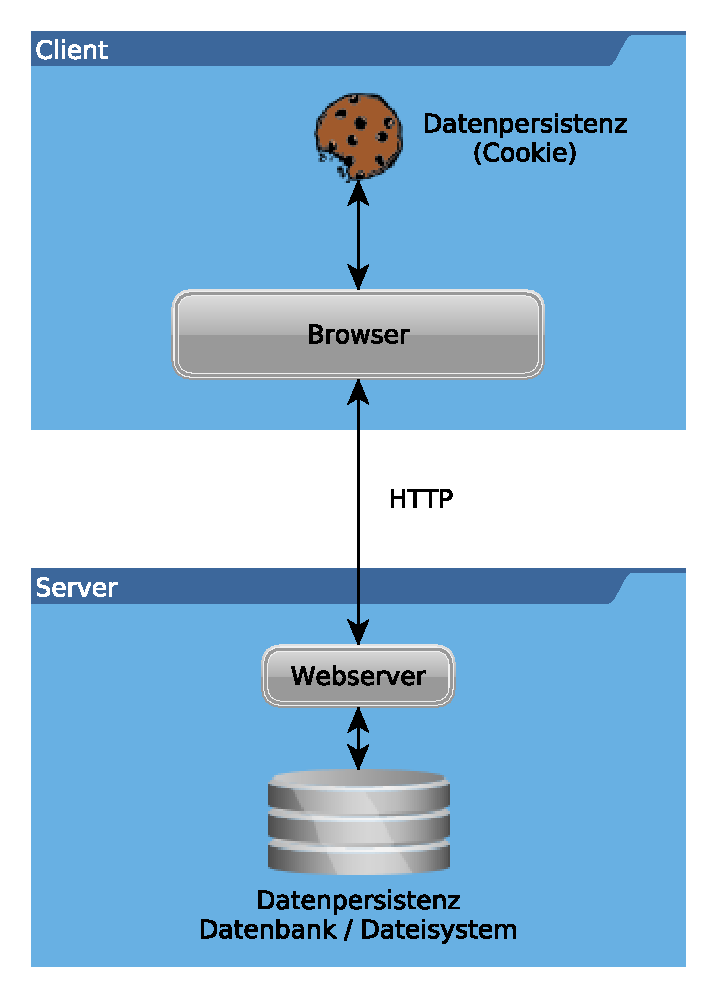
\includegraphics[scale=0.8]{images/Webapps}
	\caption[Schematische Darstellung einer WebApp]{Schematische Darstellung einer WebApp}
	\label{Webapps}
\end{figure}

Ebenso wird eine aktive Internetverbindung benötigt wenn die App ausschließlich online zur Verfügung steht. Um dies zu umgehen wurde in HTML5 verschiedenen Möglichkeiten eingebaut um Code und Daten lokal zwischenzuspeichern zu können. Dadurch, dass die App auf eine Webserver gehostet ist, kann diese schnell veröffentlicht und aktualisiert werden. Wenn der Nutzer die Anwendung mit einer aktiven Internet Verbindung öffnet, aktualisiert sich die App automatisch. 

Sofern es sich bei der Anwendung nicht um eine sogenannte \textbf{Single Page Application} handelt, wodurch die Berechnungen auf den Client ausgelagert werden würden, übernimmt der Server, welcher die Anwendung hostet einen Großteil der Datenverarbeitung. Dann dient der Client lediglich der Anzeige der Anwendung und Interaktion mit dem Nutzer.

Der Nachteil dadurch das die App im Webbrowser läuft ist, dass man nur Zugriff auf die Funktionen hat, die der verwendete Browser bietet. Da ein Webbrowser nicht zwangsläufig auf einem mobilen Gerät mit diversen Sensoren laufen muss, ist der Zugriff auf die gängigen Sensoren in einem mobilen Endgerät meinst sehr eingeschränkt. Auf Grund dessen muss man sich bei der Web-App Entwicklung meist auf Kamera, Datenpersistenz und GPS beschränken.

Durch die Zentralisierung der App sieht diese auf jedem Gerät gleich aus. Dies erscheint im ersten Augenblick positiv, der Benutzer jedoch ist an das Bedienkonzept seines Betriebssystems gewohnt, wodurch Apps welche nicht auf das Betriebssystem zugeschnitten sind meist keinen sehr großen Anklang bei den Nutzern findet. 

\todo{inhalt des links mit reinbringen. link im kommentar}%https://de.wikipedia.org/wiki/Webanwendung#/media/File:Webanwendung_client_server_01.png

\todo{package.json erklären}
\todo{View, Controller, Fachwörter erklären}
\todo{Ionic - Cordova, Proxys zum Debuggen im Browser - Das CORS-Problem}
\paragraph{Hybride Apps}\label{Hybride Apps} basieren wie auch die Web-Apps auf den Webtechnologien HTML5, CSS und JavaScript. Laufen aber im Gegensatz zu dem Web-Apps in einem mitgelieferten Minibrowser(Webview Container).

\begin{figure}[H]
	\centering
	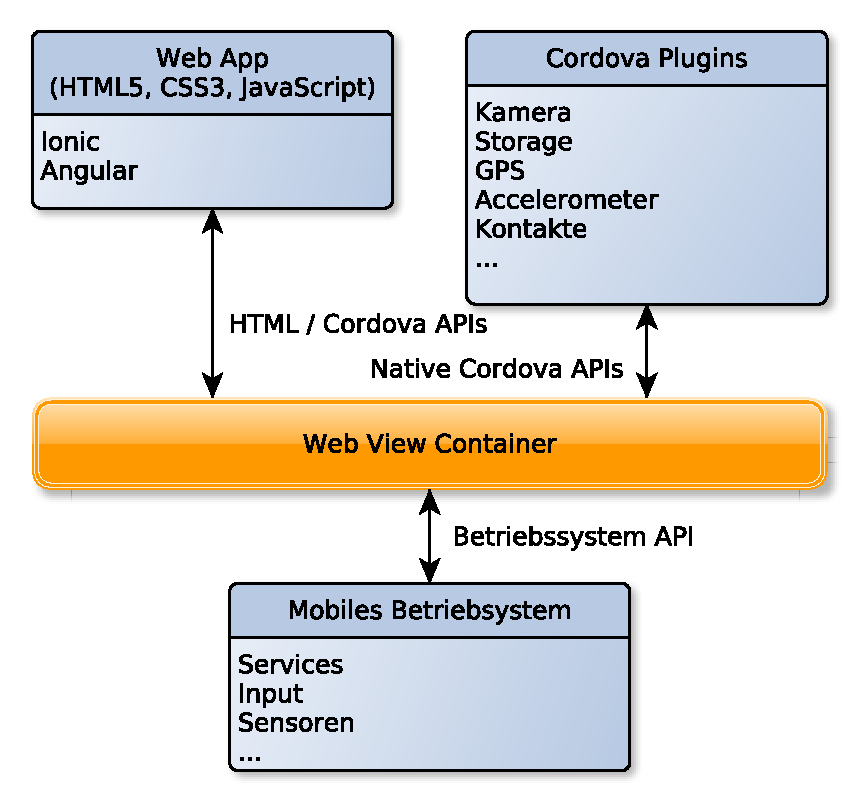
\includegraphics[scale=0.8]{images/IonicCordova}
	\caption[Aufbau des Ionic-Cordova Frameworks]{Aufbau des Ionic-Cordova Frameworks}
	\label{IonicCordova}
\end{figure}

Dieser Container ist in einer nativen App eingebettet was den Zugriff auf die System APIs des Geräts erlaubt. Durch das einbetten von nativen Code ist der Zugriff auf alle vom Betriebssystem zur Verfügung gestellten Funktionen möglich. wie z.b. GPS, Kamera, Betriebssystem Benachrichtigungen und die verschiedenen Sensoren(Beschleunigung, Umgebungslicht, Hall, Gyroskop,...). 

Da die Anwendung im Herzen eine Internetseite ist, ist es implizit möglich diese unter einer URL zu veröffentlichen und wie eine Web-App zu behandeln. Dann jedoch auch mit den Einschränkungen die diese bietet.

Für den Entwickler sehr angenehm sind oft angebotene "Live-View" Technologien. Diese erlauben durch speichern einer HTML oder JavaScript Projektdatei ein neu laden der App im Webbrowser zu initiieren. Dies bietet ein schnelles Designen der Oberfläche und implementieren grundlegender Funktionen. System eigene Funktionen müssen jedoch auf einem Gerät oder im Emulator getestet werden. Hierzu ist dann compilieren, packen und ausliefern notwendig, was etwas Zeit benötigt.

Ionic machts für jedes Gerät individuell.....

\todo{Wikipediaartikel is nochmal anders beschrieben} %https://de.wikipedia.org/wiki/Mobile_App#Hybrid-Apps

\paragraph{Native Cross Plattform Apps} mit gemeinsamer Codebasis verspricht \textbf{Xamarin}, ein Projekt das auf der quellen-offenen Implementierung von Microsofts .NET Framework, Mono basiert \cite{MONO16}. Mittels des Mono Frameworks ist es möglich C\# Code auf verschiedenen Betriebssystemen laufen zu lassen. Der geschriebene Code wird dann beim Bauvorgang der App in Nativen Code umgesetzt. Es fällt somit im Gegensatz zu den Hybriden Apps, das Framework auf dem Endgerät weg, wodurch Rechenkapazität gespart wird. Was diese Plattform vor allem für rechenintensive Anwendungen interessant macht.

\begin{figure}[H]
	\centering
	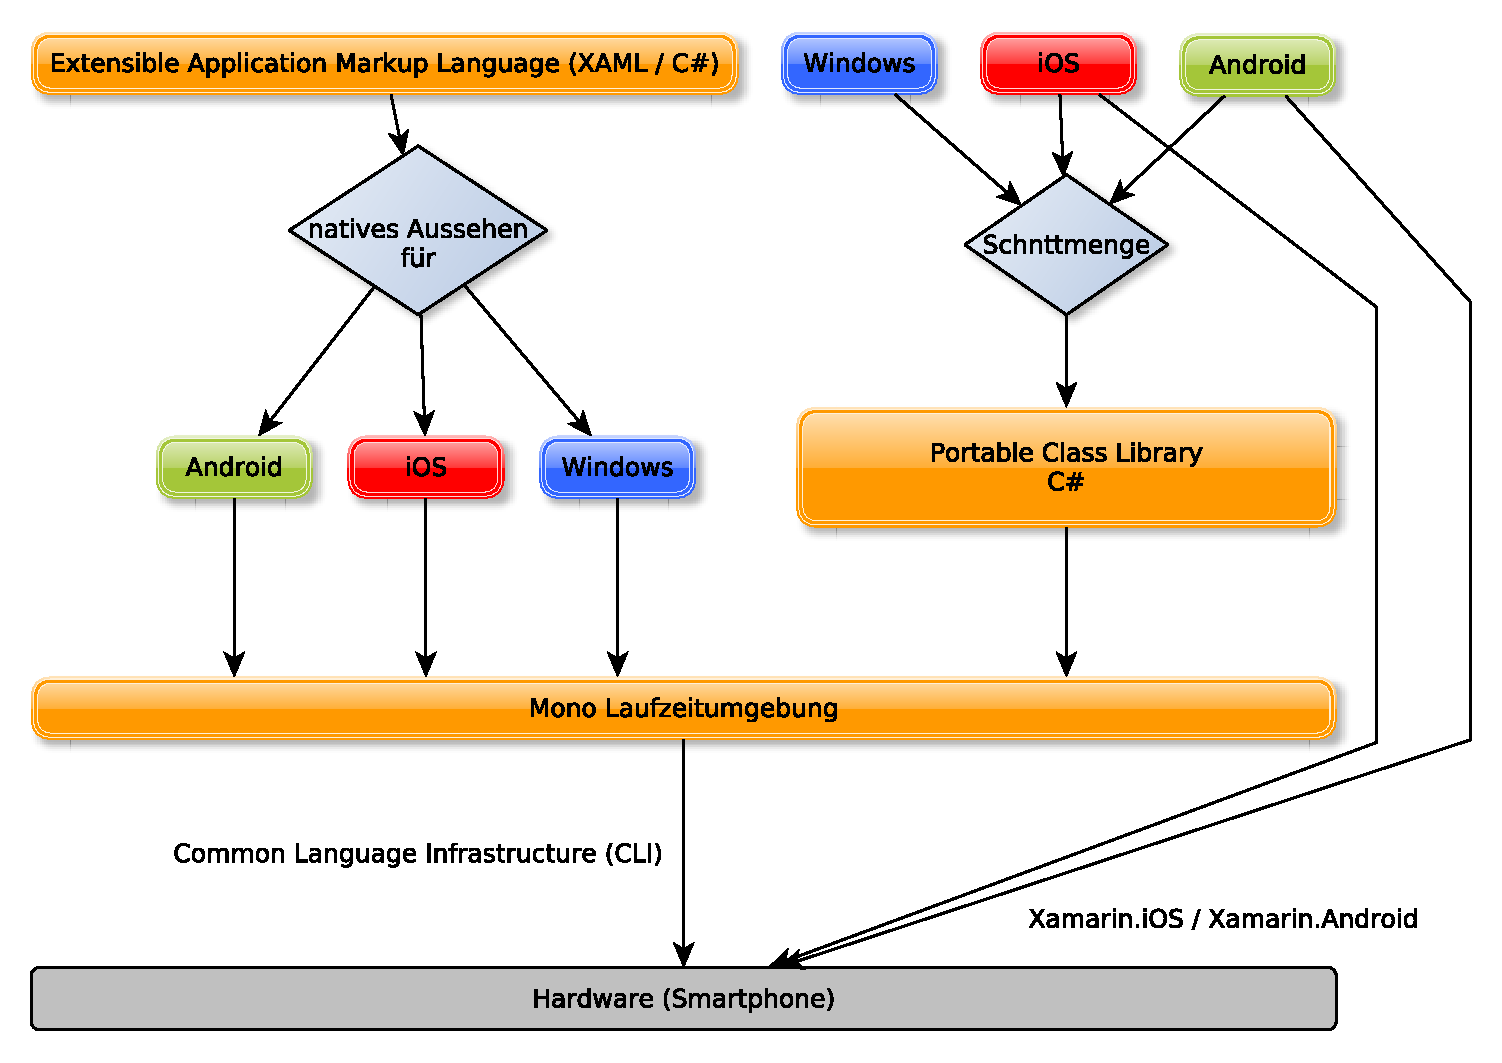
\includegraphics[scale=0.58]{images/Xamarin}
	\caption[Aufbau des Xamarin Frameworks]{Aufbau des Xamarin Frameworks}
	\label{XamarinBild}
\end{figure}

Bei der Erstellung einer Cross Plattform App mittels Xamarin muss man zuerst festlegen, auf welchen Betriebssystemen diese später laufen soll. Aus dieser Auswahl wird eine Schnittmenge der Funktionen gebildet die zur Verfügung stehen und eine sogenannte \textbf{Portable Class Library} erzeugt. Diese fungiert dann als einheitliche Schnittstelle bei Api aufrufen an das Betriebssystem.

Es sind jedoch nur die Funktionen Plattform-übergreifend nutzbar, welche von allen ausgewählten Betriebssystemen angeboten werden und von Mono implementiert sind. 
Sollte der Entwickler Zugriff auf System-eigene Funktionen benötigen, welche nicht von Mono abgedeckt werden, hat er mit Xamarin.iOS und Xamarin.Android die Möglichkeit alle System-eigenen Funktionen verwenden zu können. Zur Vereinheitlichung unter einer gemeinsamen GUI ist es dann aber nötig die Funktion für jedes Betriebssystem separat zu entwickeln und zu pflegen.

Mittels Xamarin.Forms ist es möglich die GUI der App Plattform-übergreifend zu gestalten. Hierzu wird die Oberfläche mittels einer eigenen, XML ähnlichen, Sprache namens \textbf{Extensible Application Markup Language (kurz XAML)} beschrieben. Die so spezifizierten Views werden dann auf die einzelnen Betriebssysteme zugeschnitten, um dem Anwender eine gewohnte Umgebung zu bieten. 

\section{Software Analyse}

